\documentclass{paper}

%\usepackage{times}
\usepackage{epsfig}
\usepackage{graphicx}
\usepackage{amsmath}
\usepackage{amssymb}
\usepackage{color}
\usepackage{caption}
\usepackage{subcaption}


% load package with ``framed'' and ``numbered'' option.
%\usepackage[framed,numbered,autolinebreaks,useliterate]{mcode}

% something NOT relevant to the usage of the package.
\setlength{\parindent}{0pt}
\setlength{\parskip}{18pt}
\graphicspath{{images/}}


\usepackage[latin1]{inputenc} 
\usepackage[T1]{fontenc} 


\usepackage{listings} 
\lstset{% 
   language=Matlab, 
   basicstyle=\small\ttfamily, 
} 



\title{Assignment 2}



\author{Jenni Simon\\09-116-005}
% //////////////////////////////////////////////////


\begin{document}



\maketitle


% Add figures:
%\begin{figure}[t]
%%\begin{center}
%\quad\quad   \includegraphics[width=1\linewidth]{ass2}
%%\end{center}
%
%\label{fig:performance}
%\end{figure}

\section*{Photometric Stereo}



\paragraph{1. Epipolar lines estimation}
The first part of this assignment is concerned with estimating the fundamental matrix $\mathbf{F}$ from user-specified corresponding points in two images of the Zytglogge in Bern (See figure \ref{fig:zytglogge}) using the eight-point algorithm. 

\begin{figure*}[h!]
    \centering
    \begin{subfigure}[]{0.5\textwidth}
        \centering
        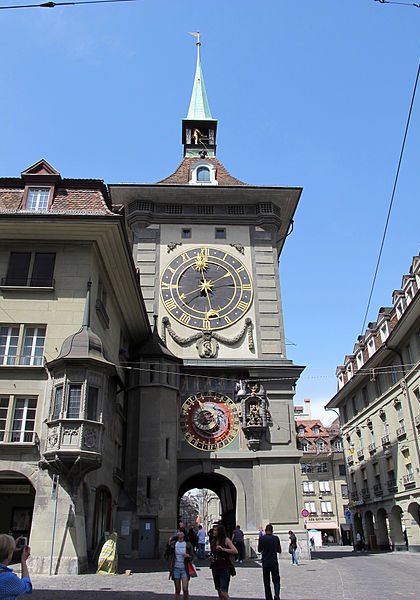
\includegraphics[height=2.5in]{left.jpg}
    \end{subfigure}%
    ~ 
    \begin{subfigure}[]{0.5\textwidth}
        \centering
        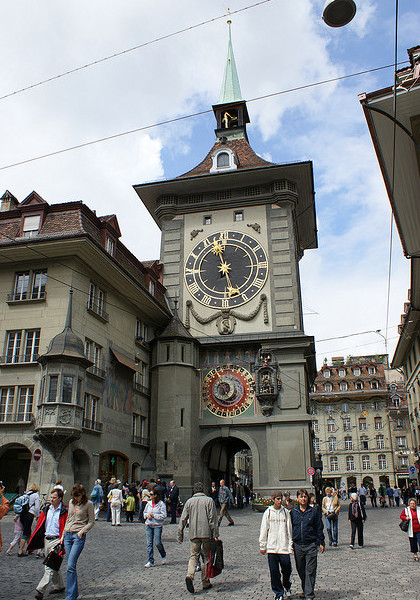
\includegraphics[height=2.5in]{right.jpg}
    \end{subfigure}
    \caption{Input images of the Zytglogge taken from different  positions.}
\label{fig:zytglogge}
\end{figure*}


\subparagraph{Gathering corresponding points}
In order to estimate $\mathbf{F}$, a minimum of eight corresponding points in both images are necessary. The user is therefore asked to input eight correspondences between the left and right images displayed to him. For every correspondence the user is asked to first click the point in the left image and then click the corresponding point in the right image. The chosen points are marked such that points belonging to a pair have the same color and different pairs have different color (figure \ref{fig:corresp}). It should be noted the the eight points should not be co-planar for the algorithm to work properly.
\begin{figure*}[h!]
   \centering
   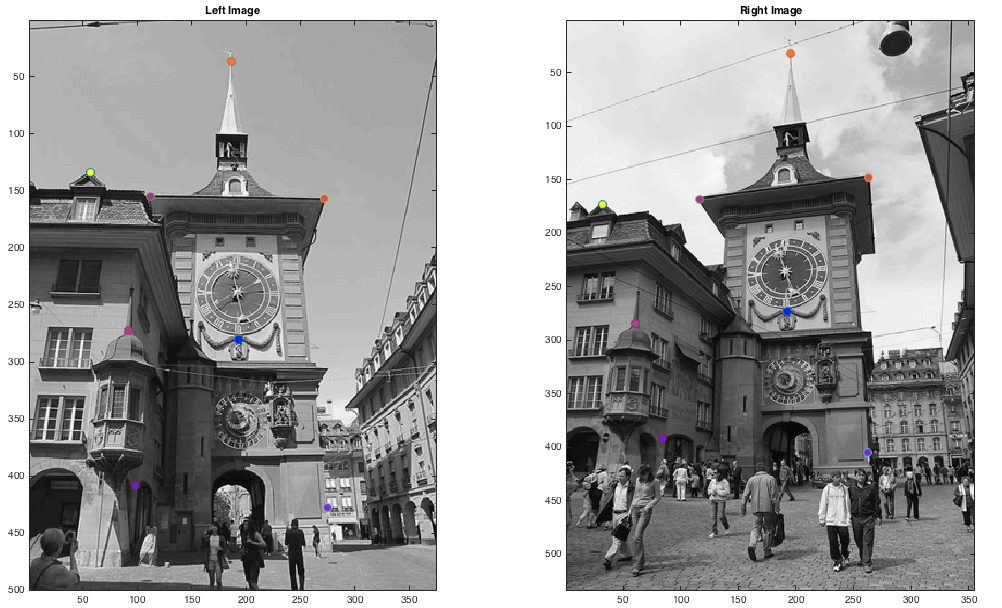
\includegraphics[height=2.8in]{corresp}
        \caption{Correspondances specified by the user.}
\label{fig:corresp}
\end{figure*}

\subparagraph{Algorithm}
Let $x_{i1}$ and $x_{i2}$ be homogeneous image-coordinates $x=(u,v,1)$ of  the $i^{th}$ matched pair in the left and right image respectively. The fundamental matrix $\mathbf{F}$ satisfies the condition
\begin{equation} 
x_{i1}^T\mathbf{F}x_{i2} = 0
\end{equation}
If we set $f^T=[F_{11},F_{12},F_{13},F_{21},F_{22},F_{23},F_{31},F_{32},F_{33}]$ as the vectorisation of $\mathbf{F}$, we can express the condition as inner product:
\begin{equation} 
[u_{i2}u_{i1}, u_{i2}v_{i1}, u_{i2}, v_{i2}u_{i1}, v_{i2}v_{i1}, v_{i2}, u_{i1}, v_{i1}, 1]\cdot f = 0
\end{equation}
Given $N$ matching points we can further stack them in an $N\times9$ matrix $A$ and arrive at the linear system 
\begin{equation} 
A\cdot f = 0
\label{eq:linsys}
\end{equation}
As the solutions are ambiguous up to scale, solving for $f$ while avoiding the trivial solution $f=0$ is a minimum direction problem (constrain $\vline f\vline=1$) and can be solved by looking at the SVD of $A=USV^T$. The vector $f$ is then given by the last column of $V$.
In general, the resulting fundamental matrix $\mathbf{F}$ (obtained by reshaping $f$) will not be of rank two. To enforce the singularity constraint on $\mathbf{F}$ we therefore take the SVD of $\mathbf{F}$, set the last singular value in $S$ to zero and multiply the factors out again to get an $\mathbf{F}$ of rank two.
To improve the quality of the solution, the data should be normalised prior to the computations. The reason for this is that some of the entries of $A$ can be on the order of $1$ while others can be on the order of $w\cdot h$, where $w$ and $h$ are the dimensions of the input images. We therefore transform the points in image 1 and 2 with transformation-matrices $T_1$, and $T_2$, such that the transformed points $x_{i1}'=T_1x_{i1}$ and $x_{i2}'=T_1x_{i2}$ have a mean value of zero and their mean distance to the origin is $\sqrt{2}$.

\subparagraph{Results}

The following results were obtained using 8 matching pairs. $\mathbf{F}^{8}$ is the estimated fundamental matrix and $e^{8}_{left}$, $e^{8}_{right}$ are the estimated epipoles in the left and right image respectively (epipoles were divided by homogenous cordinate):
\begin{align}
\mathbf{F^{8}}= \left[ \begin{array}{ccc}
0.0 & 0.0 & -0.008\\
0.0 & 0.0 & -0.008 \\
0.005 & 0.008 & 0.426 \\
\end{array} \right] \nonumber 
&& \mathbf{e^{8}_{left}}=\left[ \begin{array}{c}
-715 \\
430 \\
1\\
\end{array} \right] \nonumber 
&& \mathbf{e^{8}_{right}}=\left[ \begin{array}{c}
-369 \\
392 \\
1\\
\end{array} \right] \nonumber 
\end{align}
The epipoles were computed as $\mathbf{e_{left}}=\mathbf{null}(\mathbf{F})$ and $\mathbf{e_{right}}=\mathbf{null}(\mathbf{F}^T)$.
Looking at the coordinates of the epipoles, we observe an obvious error in the estimate. While the result for  the right epipole is more or less plausible, the left epipole can clearly not be correct, as the x-coordinate would have to be positive. A possible explanation for this is that the algorithm is sensitive to noise in the matchings, especially when there are only few matches. In order to test this suspicion and the robustness of the algorithm, I repeated the experiment with 16 matches: 
\begin{align}
\mathbf{F^{16}}= \left[ \begin{array}{ccc}
0.0 & 0.0 & 0.003\\
0.0 & 0.0 & 0.007 \\
-0.001 & -0.007 & -0.321 \\
\end{array} \right] \nonumber 
&& \mathbf{e^{16}_{left}}=\left[ \begin{array}{c}
7514 \\
-974 \\
1\\
\end{array} \right] \nonumber 
&& \mathbf{e^{16}_{right}}=\left[ \begin{array}{c}
-1141 \\
577 \\
1\\
\end{array} \right] \nonumber 
\end{align}
The fundamental matrix obtained in this case is quite different and the epipoles more plausible as well. However, the homogeneous coordinates in all cases were very small (likely due to the images being taken from relatively similar positions), indicating another possible explanation for the wrong epipoles. Experiments with even more matches showed only small changes in the fundamental matrix while still sometimes showing inplausible epipoles.

Figure \ref{fig:epilines} shows epipolar lines in the right image corresponding to points indicated in the left image. The fundamental matrix in this case was estimated using the eight points from figure \ref{fig:corresp}.

\begin{figure*}[h!]
   \centering
   \includegraphics[height=2.8in]{epilines}
        \caption{Epipolar lines in the right image corresponding to the image-points in the left image.}
\label{fig:epilines}
\end{figure*}


\paragraph{2. Model reconstruction}
The second part of the assignment is concerned with estimating the essential matrix, the rotation and translation of  the to views and finally reconstructing 3D-points from dense correspondences between two images of a cow.

\begin{figure*}[h!]
    \centering
    \begin{subfigure}[]{0.5\textwidth}
        \centering
        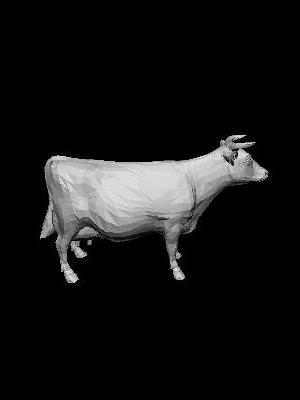
\includegraphics[height=2.5in]{leftCow.jpg}
    \end{subfigure}%
    ~ 
    \begin{subfigure}[]{0.5\textwidth}
        \centering
        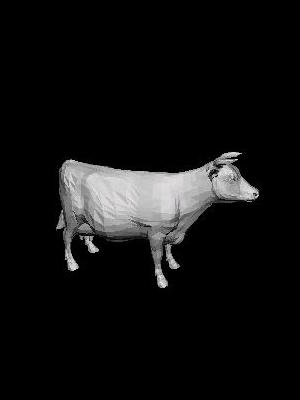
\includegraphics[height=2.5in]{rightCow.jpg}
    \end{subfigure}
    \caption{Synthetic input images for the cow.}
\label{fig:cow}
\end{figure*}

\subparagraph{Estimating the essential-matrix} 
The essential matrix $\mathbf{E}$ can be computed from the fundamental matrix and the intrinsic matrices $\Lambda_1$ and $\Lambda_2$ of the left and right cameras via:
\begin{equation} 
\mathbf{E} =\Lambda_2^T \mathbf{F} \Lambda_1
\label{eq:essential}
\end{equation}
In our case $\Lambda_1=\Lambda_2=\Lambda$.
We were given the true intrinsic parameters in the form of a matrix $K$ and the focal length $f=f_r=f_l$ of the camera. The relation between $K$ and $\Lambda$ is given by:
\begin{align}
K= \left[ \begin{array}{ccc}
m_x & \gamma & u_0\\
0 & m_y & v_0 \\
0 & 0 & 1 \\
\end{array} \right] \nonumber 
&& \Lambda= \left[ \begin{array}{ccc}
f\cdot m_x & \gamma & u_0\\
0 & f\cdot m_y & v_0 \\
0 & 0 & 1 \\
\end{array} \right] \nonumber 
\end{align}
We can therefore compute the fundamental matrix using the eight-point algorithm and then use equation \ref{eq:essential} to compute the essential matrix. The resulting estimate is:
\begin{align}
\mathbf{E}= \left[ \begin{array}{ccc}
-0.008 & -2.144 & -0.881\\
-0.04 & 0.301 & -6.283 \\
0.005 & 5.936 & 0 \\
\end{array} \right] \nonumber 
\end{align}

\subparagraph{Estimating the rotation and translation}
Given the essential matrix we are able to recover the rotation and translation of one camera to the other by decomposing the essential matrix $\mathbf{E}$. We will set the rotation matrix of the left camera to the identity and the translation vector to zero.
To estimate the transformations for the right camera, let $\mathbf{E}=USV^T$ be the SVD of $\mathbf{E}$ and let $W$ be given as:
\begin{align}
W= \left[ \begin{array}{ccc}
0 & -1 & 0\\
1 & 0 & 0 \\
0 & 0 & 1 \\
\end{array} \right] \nonumber 
\end{align}
We can then compute possible rotations and translations as:
\begin{equation} 
R_1 = UW^{-1}V^T
\qquad
R_2 = UWV^T
\end{equation}
\begin{equation} 
T_\times = USWU^T
\qquad
t_2 = -t_1
\end{equation}
Where $T_\times$ and $t_1$ is given by:
\begin{align}
T_\times = \left[ \begin{array}{ccc}
0 & -t_z & t_y\\
t_z & 0 & -t_x \\
-t_y & t_x & 0 \\
\end{array} \right] \nonumber 
&& t_1= \left[ \begin{array}{c}
t_x\\
t_y \\
t_z \\
\end{array} \right] \nonumber 
\end{align}
From all the possible combinations of rotations and translations, we can find the correct one by inferring the 3d-position of a matched pair (as described in the next section) and checking in which of the four possible combinations the projected 3d-position can be seen by both cameras. It should be noted however that we can not recover the scale of the translation vector and therefore constrain it to be unit length.

The ground-truth rotation and translations provided with the synthetic input images allows us to verify our results. In order to compare them however we have to translate them to a common frame of reference. We choose the left camera's orientation as frame of reference. Let $R_r$ and $R_l$ be the ground-truth right and left rotations and $t_r$, $t_l$ be the translations. The ground truth rotations $R'$ and translation $t'$ of the right camera relative to the left camera is then given by:
\begin{align}
R' = R_r^{-1}R_l = \left[ \begin{array}{ccc}
0.929 & 0.138 & -0.345 \\
-0.129 & 0.99 & 0.048 \\
0.348 & 0 & 0.937 \\
\end{array} \right]; \nonumber 
&& t'= R_r^{-1}(t_r-t_l) = \left[ \begin{array}{c}
1.857\\
-0.259 \\
0.696 \\
\end{array} \right] \nonumber 
\end{align}
The estimated resulting from our method is given by (scaling $t$ to the same length for better comparison):
\begin{align}
R = \left[ \begin{array}{ccc}
0.928 & 0.138 & -0.345 \\
-0.129 & 0.99 & 0.049 \\
0.349 & 0 & 0.937 \\
\end{array} \right]; \nonumber 
&& t= \left[ \begin{array}{c}
1.861\\
-0.261 \\
0.685 \\
\end{array} \right] \nonumber 
\end{align}
A comparison of the results shows that we were able to accurately recover the rotation and translation with the described method.


\subparagraph{Reconstructing 3D}
Having recovered the transformations between the camera positions we can now recover 3d-positions for all the matches (up to scale).
Let $\mathbf{P_i}=\left[ R_i, t_i \right] $ be the projection matrix for image $i$. The image coordinates $q_i=(x_i,y_i,1)$  and 3d-positions $p=(u,v,w,1)$ are related by
\begin{equation}
\lambda_i q_i = \Lambda_i \mathbf{P_i} p
\end{equation}
for some $\lambda_i$. By pre-multiplying both sides with the inverse of the intrinsic matrix $\Lambda_i$ and writing $q_i'=\Lambda_i^{-1} q_i$ we get:
\begin{equation}
\lambda_i q_i' =  \mathbf{P_i} p
\label{eq:rec}
\end{equation}
We can eliminate the unknown $\lambda_i$ by expressing it in terms of $\mathbf{P_i}$ and $p$ as $\lambda_i=\mathbf{P_i}(3,:)\cdot p$. 
Substituting $\lambda_i$ in equation \ref{eq:rec} we can eliminate the last row of this equation and are left with two equations for the three unknowns per image point. As we have two images, we therefore have four equations for each of the three unknown 3d-coordinates per match. We can therefore solve for the unknown $p$ by solving a linear system $\mathbf{A}\mathbf{p}=\mathbf{b}$, where $\mathbf{p}$ is a vector of all the unknown $p$'s and  $\mathbf{A}$ and $\mathbf{b}$ encode the equations (For details please refer to the code).
\begin{figure*}[h!]
    \centering
    \begin{subfigure}[]{0.75\textwidth}
        \centering
        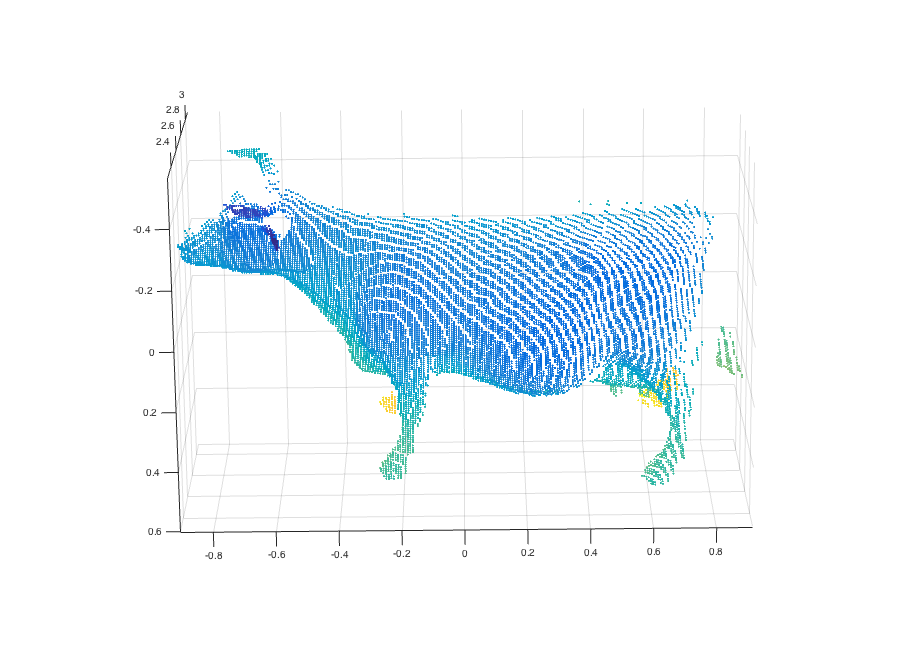
\includegraphics[width=\textwidth]{cow3d1}
    \end{subfigure}
    \begin{subfigure}[]{0.8\textwidth}
        \centering
        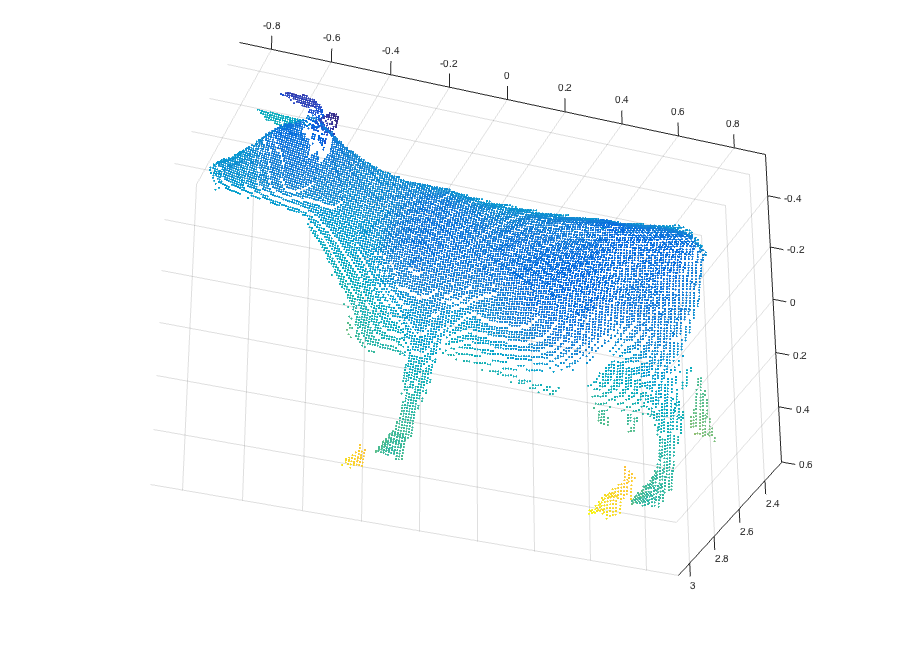
\includegraphics[width=\textwidth]{cow3d2}
    \end{subfigure}
    \caption{Results of 3d-reconstruction.}
\label{fig:cow3d}
\end{figure*}
\subparagraph{Discussion} Figure \ref{fig:cow3d} shows the resulting 3d-point cloud. We observe that contrary to the first part of the assignment, where we only had few and noisy correspondences, the method works very well in the case of dense correspondences between the two images. This has been shown both by comparing to the ground truth transformation matrices and the visual results of the reconstruction.


%\begin{figure*}[h!]
%    \centering
%    \begin{subfigure}[]{0.33\textwidth}
%        \centering
%        \includegraphics[height=1.2in]{}
%    \end{subfigure}%
%    ~ 
%    \begin{subfigure}[]{0.33\textwidth}
%        \centering
%        \includegraphics[height=1.2in]{}
%    \end{subfigure}
%    \caption{Recovered gray albedo}    
%\label{fig:GA}
%\end{figure*}

 \end{document}